\documentclass{article}

\PassOptionsToPackage{numbers,sort&compress}{natbib}
\usepackage[preprint]{neurips}
\usepackage[utf8]{inputenc}
\usepackage[T1]{fontenc}
\usepackage{hyperref}
\usepackage{url}
\usepackage{booktabs}
\usepackage{amsfonts}
\usepackage{nicefrac}
\usepackage{microtype}
\usepackage{xcolor}
\usepackage{graphicx}
\usepackage{subcaption}
\usepackage{multirow}
\usepackage{array}
\usepackage{float}
\usepackage{adjustbox}
\usepackage{amsthm}
\usepackage{amsmath}
\usepackage{amssymb}
\usepackage{mathtools}
\usepackage{enumitem}
\usepackage{algorithm}
\usepackage{algpseudocode}
\usepackage{bbm}

\title{PRISM: Post-hoc Domain Generalization via Structural Risk Minimization over Hidden-Subpopulation Regret}
\author{Anonymous Authors}

\newtheorem{theorem}{Theorem}
\newtheorem{proposition}{Proposition}
\newtheorem{lemma}{Lemma}
\newtheorem{corollary}{Corollary}
\newtheorem{definition}{Definition}
\newtheorem{assumption}{Assumption}
\newtheorem{remark}{Remark}

\newcommand{\RR}{\mathbb{R}}
\newcommand{\EE}{\mathbb{E}}
\newcommand{\PP}{\mathbb{P}}
\newcommand{\cA}{\mathcal{A}}
\newcommand{\cC}{\mathcal{C}}
\newcommand{\cD}{\mathcal{D}}
\newcommand{\cG}{\mathcal{G}}
\newcommand{\cI}{\mathcal{I}}
\newcommand{\cQ}{\mathcal{Q}}
\newcommand{\cR}{\mathcal{R}}
\newcommand{\cS}{\mathcal{S}}
\newcommand{\cT}{\mathcal{T}}
\newcommand{\cU}{\mathcal{U}}
\newcommand{\cV}{\mathcal{V}}
\newcommand{\argmin}{\operatorname*{arg\,min}}
\newcommand{\argmax}{\operatorname*{arg\,max}}
\newcommand{\CVaR}{\operatorname{CVaR}}
\newcommand{\Top}{\operatorname{Top}}
\newcommand{\KL}{\operatorname{KL}}
\newcommand{\simplex}{\Delta}
\newcommand{\TBD}{\textbf{TBD}}
\newcommand{\prism}{\textup{\textsc{PRISM}}}
\newcommand{\swad}{\textup{\textsc{SWAD}}}
\newcommand{\diwa}{\textup{\textsc{DiWA}}}
\newcommand{\miro}{\textup{\textsc{MIRO}}}
\newcommand{\erm}{\textup{\textsc{ERM}}}
\newcommand{\iid}{i.i.d.}
\newcommand{\ood}{OOD}
\newcommand{\norm}[1]{\left\lVert #1 \right\rVert}
\newcommand{\braces}[1]{\left\{ #1 \right\}}
\newcommand{\paren}[1]{\left( #1 \right)}
\newcommand{\bracks}[1]{\left[ #1 \right]}
\newcommand{\loss}{\ell}
\newcommand{\1}{\mathbbm{1}}

\begin{document}

\maketitle

\begin{abstract}
Single-run post-hoc selection is one of the most practical routes to domain generalization because it can be attached to a strong empirical-risk-minimization pipeline without retraining. Existing post-hoc selectors often leave one important step outside the theorem: they optimize a selector within one hand-chosen trajectory family, but the family itself is determined by validation heuristics or manual tuning. This paper proposes \textbf{\prism{}} (\textbf{P}ost-hoc \textbf{R}egret on \textbf{I}mplicit \textbf{S}ubpopulations of \textbf{M}odel soups), a domain-label-free post-hoc selector that closes this gap. \prism{} searches over a finite collection of admissible validation-defined soup families and chooses the final deployable soup by minimizing hidden-subpopulation regret plus an explicit structural-risk penalty. The scored action is always the deployed object: a uniform soup over a subset of dense checkpoints from one run. We prove an exact top-$\alpha$ / empirical-\(\CVaR\) form of the family-indexed regret, finite termination and exact optimality of the exhaustive selector, conditional finite-sample uniform deviation over the admissible family union, an oracle inequality for the structural-risk-minimized selector, monotonic hidden-subpopulation certificates, and domination over interval-restricted subfamilies on the \prism{} certificate. The empirical section records the protocol and exact published benchmark context from prior work, while reserving structured tables for the new measurements.
\end{abstract}

\section{Introduction}

Domain generalization (DG) asks for a predictor that performs well on an unseen target environment using only source data at training time. In practice, some of the strongest DG improvements come not from changing the training algorithm, but from changing which final predictor is deployed. This is especially true in the single-run post-hoc regime: one trains a dense trajectory once, saves checkpoints, and chooses a final model after training has already ended.

That regime is attractive because it preserves the base training pipeline. It also already works. On the standard DomainBed ResNet-50 benchmark suite, a flat-minima interval selector improves the average \ood{} accuracy of \erm{} from \(63.3\) to \(66.9\) across PACS, VLCS, OfficeHome, TerraIncognita, and DomainNet \citep{cha2021swad}. Combined with a pretraining-aware regularizer, the same post-hoc selector reaches \(68.1\) \citep{cha2022miro}. In a larger multi-run diverse-weight-averaging setting with LP initialization, the reported \diwa{}$^\dagger$ configuration with uniform \(M=60\) reaches \(68.0\) \citep{rame2022diwa}. The empirical message is clear: the best final predictor is often not the last checkpoint.

Still, an important theoretical gap remains. Post-hoc selectors are usually analyzed \emph{inside} one chosen trajectory family: a contiguous interval, a low-loss window, or an anchor-screened subset. But the choice of that family is often manual or heuristic. If the theory is meant to govern the method rather than merely rationalize one subroutine, then the family choice itself should be part of the selector.

This paper proposes \prism{}, a domain-label-free post-hoc selector that does exactly that. The core idea is simple:
\begin{quote}
\textbf{Choose the deployable soup whose worst-case regret to the best feasible soup is smallest, after paying an explicit structural-risk penalty for searching a larger validation-defined family.}
\end{quote}

The hidden-subpopulation part comes from distributionally robust and worst-case subgroup reasoning \citep{duchi2021learning,li2021worstcase,hashimoto2018fairness,lahoti2020fairness}. The regret part comes from minimax-regret learning under shift \citep{agarwal2022mro}. The structural-risk-minimization part comes from finite-family model-selection logic \citep{bartlett2002rademacher}. Combining them yields a selector that is domain-label-free, deploys an actual uniform soup, and moves candidate-family choice into a theorem-governed outer minimization.

Concretely, the validation split defines a finite collection of admissible soup families indexed by low-loss width, locality threshold, and maximum soup size. For each family, \prism{} computes the exact hidden-subpopulation regret of every feasible soup on a disjoint support split. It then chooses the family-action pair with smallest empirical regret plus an analytic Occam penalty. The result is still a single deployable soup from one dense run, not a proxy, not a predictive mixture, and not a stochastic posterior.

The paper makes five contributions.
\begin{enumerate}[leftmargin=1.4em]
    \item We formulate \prism{} as a \emph{family-aware} post-hoc selector: the method chooses both the deployable soup and the searched soup family.
    \item We derive an exact top-$\alpha$ / empirical-\(\CVaR\) characterization of the family-indexed regret objective over actual soups.
    \item We prove finite termination and exact optimality of the exhaustive selector over the admissible family union, a conditional finite-sample deviation theorem, and an oracle inequality for the structural-risk-minimized selector.
    \item We prove target-regret certificates under hidden source-supported shift, monotonic robustness certificates in \(\alpha\), and domination over interval-restricted subfamilies on the \prism{} certificate.
    \item We provide a complete experimental protocol and exact published context from prior work, while leaving the new empirical tables explicitly as \TBD{} placeholders.
\end{enumerate}

\begin{figure}[t]
    \centering
    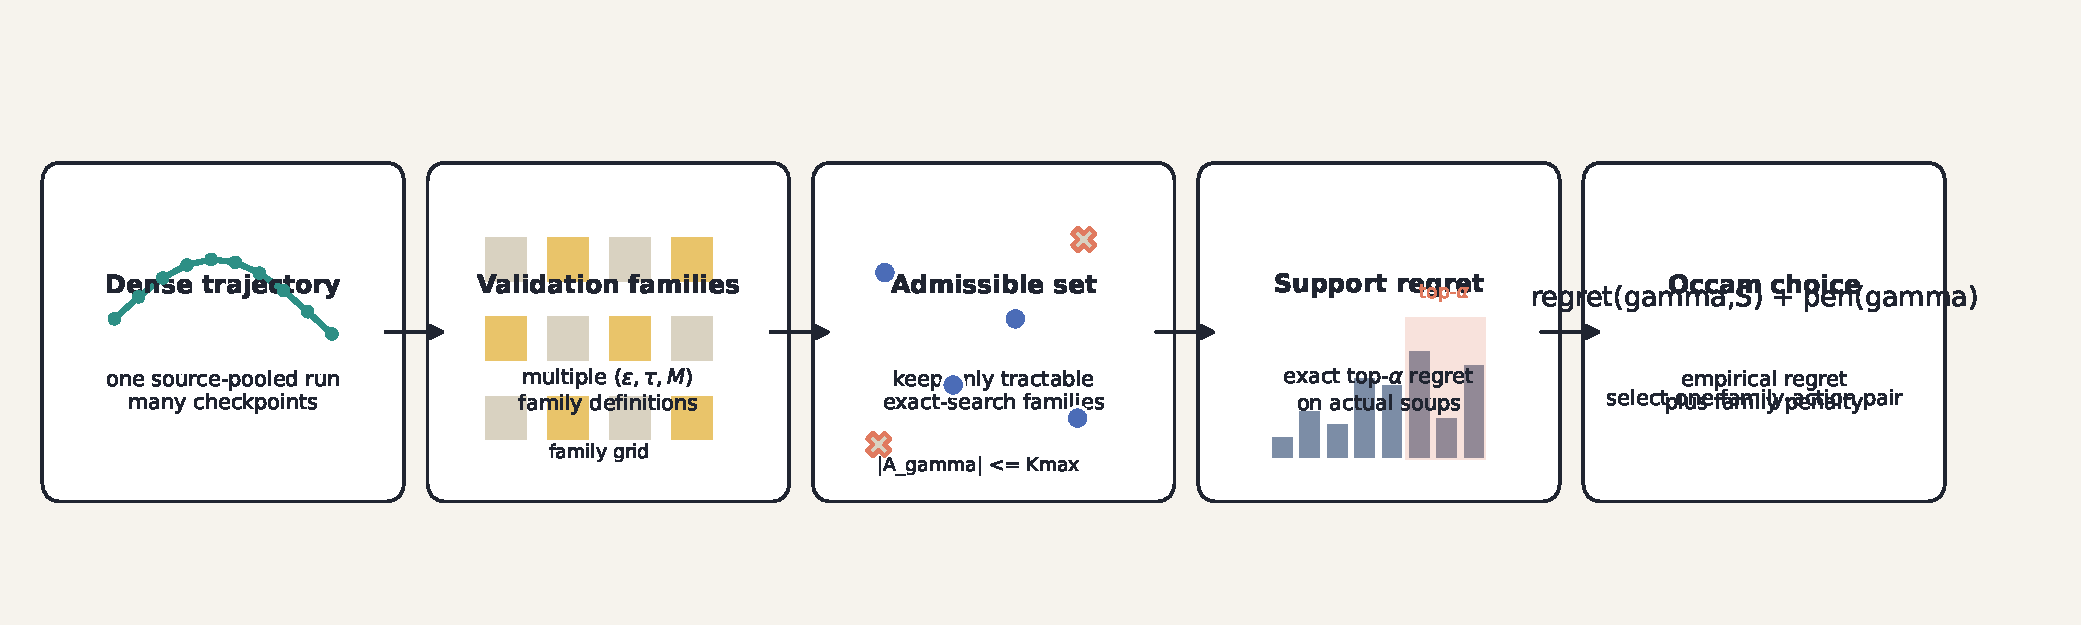
\includegraphics[width=\linewidth]{figures/prism_pipeline.pdf}
    \caption{\textbf{\prism{} at a glance.} A dense trajectory is filtered into multiple admissible soup families by validation loss, locality, and a fixed search budget. Within each family, \prism{} computes exact hidden-subpopulation regret over actual soups on a disjoint support split, then chooses the family-action pair with smallest structural-risk score.}
    \label{fig:pipeline}
\end{figure}

\section{Related Work}

\paragraph{Post-hoc DG and flat-minima selectors.}
Interval-based selectors showed that substantial DG gains can be obtained without changing the base learner \citep{cha2021swad}. Their central empirical lesson is important: contiguous late-trajectory averages can be much better than a single checkpoint. Our goal is not to discard that lesson. It is to place it inside a larger deployable family and compare it through a shared certificate.

\paragraph{Weight averaging, soups, and locality.}
Stochastic weight averaging, fast geometric ensembling, and model soups established that weight-space averages can be highly effective when the averaged models remain in a connected low-loss region \citep{izmailov2018swa,garipov2018fge,frankle2020linear,wortsman2022soups}. \diwa{} sharpened the \ood{} interpretation by emphasizing diversity, covariance, and locality trade-offs \citep{rame2022diwa}. \prism{} retains locality through validation-defined family construction, but moves the final decision rule to a regret objective over actual soups.

\paragraph{Distributional robustness and hidden subpopulations.}
Distributionally robust optimization and worst-case subgroup evaluation study predictors that perform well under reweightings of the nominal distribution \citep{duchi2016fdiv,duchi2021learning,li2021worstcase}. Group-robust and fairness-without-demographics methods use related adversarial reweightings to protect minority subpopulations without observed group labels \citep{hashimoto2018fairness,lahoti2020fairness}. \prism{} adapts that hidden-subpopulation viewpoint to post-hoc model selection.

\paragraph{Regret under shift.}
Minimax-regret learning argues that regret can be the right object under heterogeneous subgroup difficulty or uneven noise floors \citep{agarwal2022mro}. This point matters in the post-hoc setting. Worst-case raw loss can penalize a candidate because a subgroup is intrinsically hard, even if that candidate is near-optimal \emph{relative to the feasible family} on that subgroup. Regret removes the subgroup-specific floor.

\paragraph{Structural risk minimization and stability.}
Finite-family model selection relies on the principle that empirical performance should be balanced against the complexity of the searched class \citep{bartlett2002rademacher}. Stability is another route to generalization \citep{bousquet2002stability}, but in the present post-hoc setting, uniform algorithmic stability does not directly justify bootstrap variability of the final regret score. We therefore use stability only as background motivation, not as the main theorem-bearing device.

\section{Problem Setup}
\label{sec:setup}

We consider multiclass classification in the single-run post-hoc DG setting. A base learner produces dense checkpoints
\[
    \{\theta_t\}_{t=1}^{K}.
\]
Post-hoc selection uses two \emph{pooled} labeled source holdout splits:
\begin{itemize}[leftmargin=1.4em]
    \item a validation split \(\cV = \{(x_j,y_j)\}_{j=1}^{n_V}\), used only to define admissible soup families, and
    \item a support split \(\cU = \{(x_i,y_i)\}_{i=1}^{n}\), used only to compute the post-hoc selection score.
\end{itemize}
Neither split uses source-domain identities.

For checkpoint \(\theta_t\), let \(p_t(x)\in\simplex^{C-1}\) denote the predicted class-probability vector. Fix a probability floor \(\varepsilon_p\in(0,1)\). The pooled validation loss is
\begin{equation}
    L_{\cV}(\theta_t)
    \triangleq
    \frac{1}{n_V}\sum_{j=1}^{n_V}
    -\log \max\braces{p_t(x_j)_{y_j},\varepsilon_p}.
    \label{eq:val_loss}
\end{equation}
The validation-best anchor checkpoint is
\begin{equation}
    a(\cV)
    \in
    \argmin_{1\le t\le K} L_{\cV}(\theta_t).
    \label{eq:anchor}
\end{equation}

Locality is screened with a validation barrier. For a fixed interpolation grid \(\Lambda\subset[0,1]\),
\begin{equation}
    B_{\cV}\!\big(t,a(\cV)\big)
    \triangleq
    \max_{\lambda\in\Lambda}
    L_{\cV}\!\big((1-\lambda)\theta_{a(\cV)} + \lambda \theta_t\big)
    -
    \max\braces{L_{\cV}(\theta_{a(\cV)}),L_{\cV}(\theta_t)}.
    \label{eq:barrier}
\end{equation}

The structural-risk-minimization stage searches over a predeclared finite grid of family indices
\[
    \Gamma_0 \subset \RR_+ \times \RR_+ \times \mathbb{N},
\]
where \(\gamma=(\varepsilon,\tau,M)\) denotes a validation-loss width, a locality threshold, and a maximum soup size. The robustness parameter \(\alpha\in(0,1]\) is \emph{not} part of the family index: it defines the hidden-subpopulation size we aim to protect and is treated as an exogenous scientific choice.

\begin{definition}[Validation-defined candidate pool and soup family]
For \(\gamma=(\varepsilon,\tau,M)\in\Gamma_0\), define
\begin{align}
    \cC_\gamma(\cV)
    &\triangleq
    \braces{
        t :
        L_{\cV}(\theta_t)\le L_{\cV}^\star + \varepsilon,\;
        B_{\cV}\!\big(t,a(\cV)\big)\le \tau
    },
    \label{eq:candidate_pool}
    \\
    \cA_\gamma(\cV)
    &\triangleq
    \braces{
        S\subseteq \cC_\gamma(\cV) :
        1\le |S|\le M
    },
    \label{eq:action_family}
 \end{align}
where \(L_{\cV}^\star=\min_t L_{\cV}(\theta_t)\).
\end{definition}

We make tractability part of the method. Fix a global exact-search budget \(K_{\max}\in\mathbb{N}\). The admissible family index set is
\begin{equation}
    \Gamma_{\mathrm{adm}}(\cV)
    \triangleq
    \braces{
        \gamma\in\Gamma_0 :
        |\cA_\gamma(\cV)| \le K_{\max}
    }.
    \label{eq:admissible_gamma}
\end{equation}

The deployable object associated with \(S\in\cA_\gamma(\cV)\) is the uniform soup
\begin{equation}
    \bar{\theta}_S
    \triangleq
    \frac{1}{|S|}
    \sum_{t\in S}\theta_t.
    \label{eq:uniform_soup}
\end{equation}

For support example \(z_i=(x_i,y_i)\in\cU\), define the \emph{normalized} clipped action loss
\begin{equation}
    \loss_i(S)
    \triangleq
    \frac{
        -\log \max\braces{p_{\bar{\theta}_S}(x_i)_{y_i},\varepsilon_p}
    }{
        -\log \varepsilon_p
    }.
    \label{eq:normalized_loss}
\end{equation}
Hence
\begin{equation}
    0 \le \loss_i(S)\le 1
    \qquad
    \forall S,\forall i.
    \label{eq:loss_bounded}
\end{equation}

\section{PRISM: Structural-Risk-Minimized Hidden-Subpopulation Regret}
\label{sec:method}

\subsection{Family-indexed hidden-subpopulation regret}

Let \(\alpha\in(0,1]\) denote the minimum hidden-subpopulation mass of interest. Define the capped adversarial simplex
\begin{equation}
    \cQ_\alpha^n
    \triangleq
    \braces{
        q\in\simplex^n :
        q_i \le \frac{1}{\alpha n}
        \;\;\forall i
    }.
    \label{eq:capped_simplex}
\end{equation}

For every admissible family \(\gamma\in\Gamma_{\mathrm{adm}}(\cV)\) and every action \(S\in\cA_\gamma(\cV)\), define the empirical hidden-subpopulation regret
\begin{equation}
    \widehat{\Psi}^{(\gamma,\cV)}_\alpha(S;\cU)
    \triangleq
    \sup_{q\in\cQ_\alpha^n}
    \left[
        \sum_{i=1}^{n} q_i \loss_i(S)
        -
        \min_{S'\in\cA_\gamma(\cV)}
        \sum_{i=1}^{n} q_i \loss_i(S')
    \right].
    \label{eq:family_regret}
\end{equation}

This is the key alignment principle of \prism{}:
\begin{itemize}[leftmargin=1.4em]
    \item the scored object is the actual deployable soup;
    \item the witness class is exactly the same family from which that soup is drawn;
    \item and the adversary ranges over sufficiently large hidden source-supported subpopulations.
\end{itemize}

\subsection{\texorpdfstring{Exact top-\(\alpha\) and empirical-\(\CVaR\) characterization}{Exact top-alpha and empirical-CVaR characterization}}

For \(v\in\RR^n\), let \(v_{(1)}\ge \cdots \ge v_{(n)}\) denote the sorted entries. Define
\begin{equation}
    \Top_\alpha(v)
    \triangleq
    \sup_{q\in\cQ_\alpha^n}\sum_{i=1}^{n}q_i v_i.
    \label{eq:top_alpha_def}
\end{equation}

\begin{proposition}[Exact top-\(\alpha\) form]
\label{prop:top_alpha}
For any admissible family \(\gamma\in\Gamma_{\mathrm{adm}}(\cV)\) and any \(S\in\cA_\gamma(\cV)\),
\begin{equation}
    \widehat{\Psi}^{(\gamma,\cV)}_\alpha(S;\cU)
    =
    \max_{S'\in\cA_\gamma(\cV)}
    \Top_\alpha\!\big(\loss(S)-\loss(S')\big).
    \label{eq:family_top_alpha}
\end{equation}
Moreover,
\begin{equation}
    \Top_\alpha(v)
    =
    \inf_{\eta\in\RR}
    \bracks{
        \eta + \frac{1}{\alpha n}\sum_{i=1}^{n}(v_i-\eta)_+
    }.
    \label{eq:cvar_rep}
\end{equation}
Hence \(\widehat{\Psi}^{(\gamma,\cV)}_\alpha\) is an exact empirical-\(\CVaR\) regret over pairwise action gaps.
\end{proposition}

\begin{figure}[t]
    \centering
    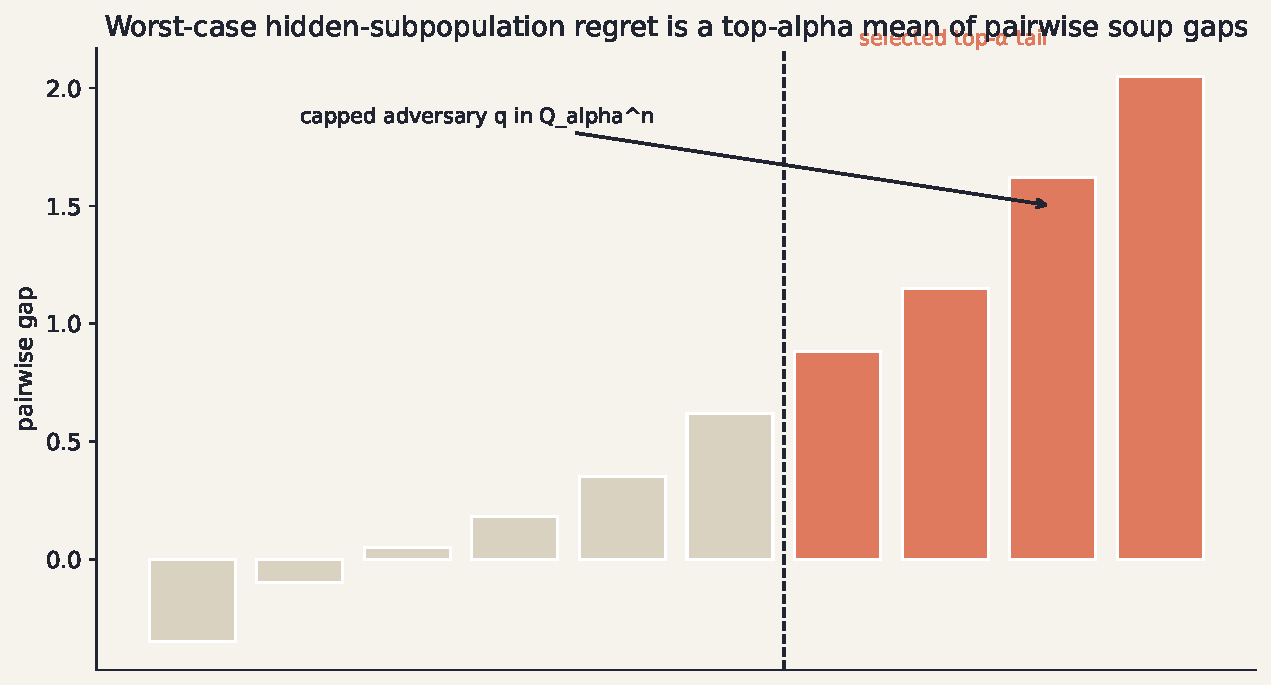
\includegraphics[width=0.88\linewidth]{figures/tail_regret_geometry.pdf}
    \caption{\textbf{Exact hidden-subpopulation geometry.} For a fixed candidate soup \(S\) and witness soup \(S'\), the capped adversary selects the highest tail of the pairwise gap vector. This is exactly the objective optimized by \prism{}, not a surrogate.}
    \label{fig:tail_geometry}
\end{figure}

\subsection{Structural risk minimization across admissible families}

We now define the outer selector. Let \(\pi_\Gamma\) be a fixed prior mass function on \(\Gamma_0\) with \(\sum_{\gamma\in\Gamma_0}\pi_\Gamma(\gamma)=1\). For a given support sample size \(n\) and confidence level \(\delta\in(0,1)\), define the family penalty
\begin{equation}
    \operatorname{pen}_{\alpha,n,\delta}(\gamma;\cV)
    \triangleq
    \left(1+\frac{1}{\alpha}\right)
    \left[
    \sqrt{
        \frac{
            2\log \frac{2(2n+1)}{\delta\,\pi_\Gamma(\gamma)}
            +
            4\log |\cA_\gamma(\cV)|
        }{n}
    }
    +
    \frac{2}{n}
    \right].
    \label{eq:penalty}
\end{equation}
This is an analytic function of \(\alpha,n,\delta,\pi_\Gamma(\gamma)\), and \(|\cA_\gamma(\cV)|\). It is not a tuned coefficient.

The \prism{} selector is
\begin{equation}
    (\widehat{\gamma}_\alpha,\widehat{S}_\alpha)
    \in
    \argmin_{\gamma\in\Gamma_{\mathrm{adm}}(\cV),\; S\in\cA_\gamma(\cV)}
    \bracks{
        \widehat{\Psi}^{(\gamma,\cV)}_\alpha(S;\cU)
        +
        \operatorname{pen}_{\alpha,n,\delta}(\gamma;\cV)
    }.
    \label{eq:prism_selector}
\end{equation}

The selector therefore balances three quantities:
\begin{itemize}[leftmargin=1.4em]
    \item hidden-subpopulation regret within a fixed family;
    \item family richness through \(|\cA_\gamma(\cV)|\);
    \item and prior complexity through \(\pi_\Gamma(\gamma)\).
\end{itemize}

\begin{figure}[t]
    \centering
    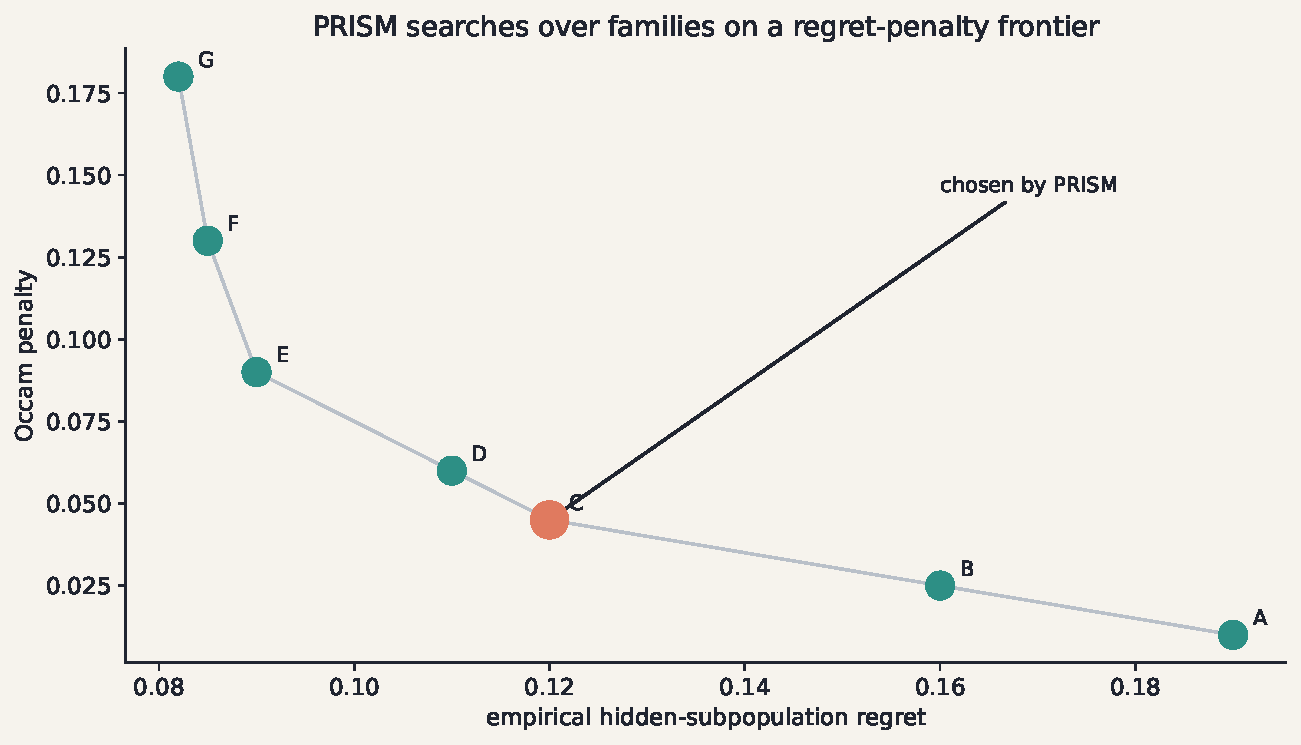
\includegraphics[width=\linewidth]{figures/family_frontier.pdf}
    \caption{\textbf{Family-aware selection frontier.} Different validation-defined soup families induce different trade-offs between empirical regret and Occam penalty. \prism{} chooses the family-action pair with smallest total score, rather than optimizing inside a hand-picked family.}
    \label{fig:frontier}
\end{figure}

\subsection{Exact exhaustive selector}

Whenever \(|\cA_\gamma(\cV)|\le K_{\max}\) for all admissible families, \prism{} uses exact exhaustive search.

\begin{algorithm}[t]
\caption{\prism{} exact family-aware post-hoc selector}
\label{alg:prism}
\begin{algorithmic}[1]
\Require Dense checkpoints \(\{\theta_t\}_{t=1}^{K}\), validation split \(\cV\), support split \(\cU\), robustness target \(\alpha\), family grid \(\Gamma_0\), prior \(\pi_\Gamma\), confidence level \(\delta\), search budget \(K_{\max}\)
\State Choose anchor \(a(\cV)\) by Eq.~\eqref{eq:anchor}
\For{each \(\gamma=(\varepsilon,\tau,M)\in\Gamma_0\)}
    \State Build \(\cC_\gamma(\cV)\) and \(\cA_\gamma(\cV)\) using Eqs.~\eqref{eq:candidate_pool}--\eqref{eq:action_family}
    \If{\(|\cA_\gamma(\cV)| > K_{\max}\)}
        \State mark \(\gamma\) inadmissible
    \Else
        \For{each \(S\in\cA_\gamma(\cV)\)}
            \State materialize \(\bar{\theta}_S\) by Eq.~\eqref{eq:uniform_soup}
            \State evaluate \(\loss_i(S)\) on \(\cU\) by Eq.~\eqref{eq:normalized_loss}
        \EndFor
        \State compute \(\widehat{\Psi}^{(\gamma,\cV)}_\alpha(S;\cU)\) for all \(S\in\cA_\gamma(\cV)\)
        \State compute family score in Eq.~\eqref{eq:prism_selector}
    \EndIf
\EndFor
\State Return the minimizer \((\widehat{\gamma}_\alpha,\widehat{S}_\alpha)\)
\end{algorithmic}
\end{algorithm}

\begin{proposition}[Finite termination and exact optimality]
\label{prop:termination}
Algorithm~\ref{alg:prism} terminates after finitely many operations and returns a global minimizer of Eq.~\eqref{eq:prism_selector}. Its total number of scored actions is
\begin{equation}
    N_{\mathrm{act}}(\cV)
    \triangleq
    \sum_{\gamma\in\Gamma_{\mathrm{adm}}(\cV)} |\cA_\gamma(\cV)|,
    \label{eq:total_actions}
\end{equation}
and its total pairwise-regret evaluation cost is
\begin{equation}
    O\!\left(
        n
        \sum_{\gamma\in\Gamma_{\mathrm{adm}}(\cV)}
        |\cA_\gamma(\cV)|^2
    \right).
    \label{eq:complexity}
\end{equation}
\end{proposition}

\begin{figure}[t]
    \centering
    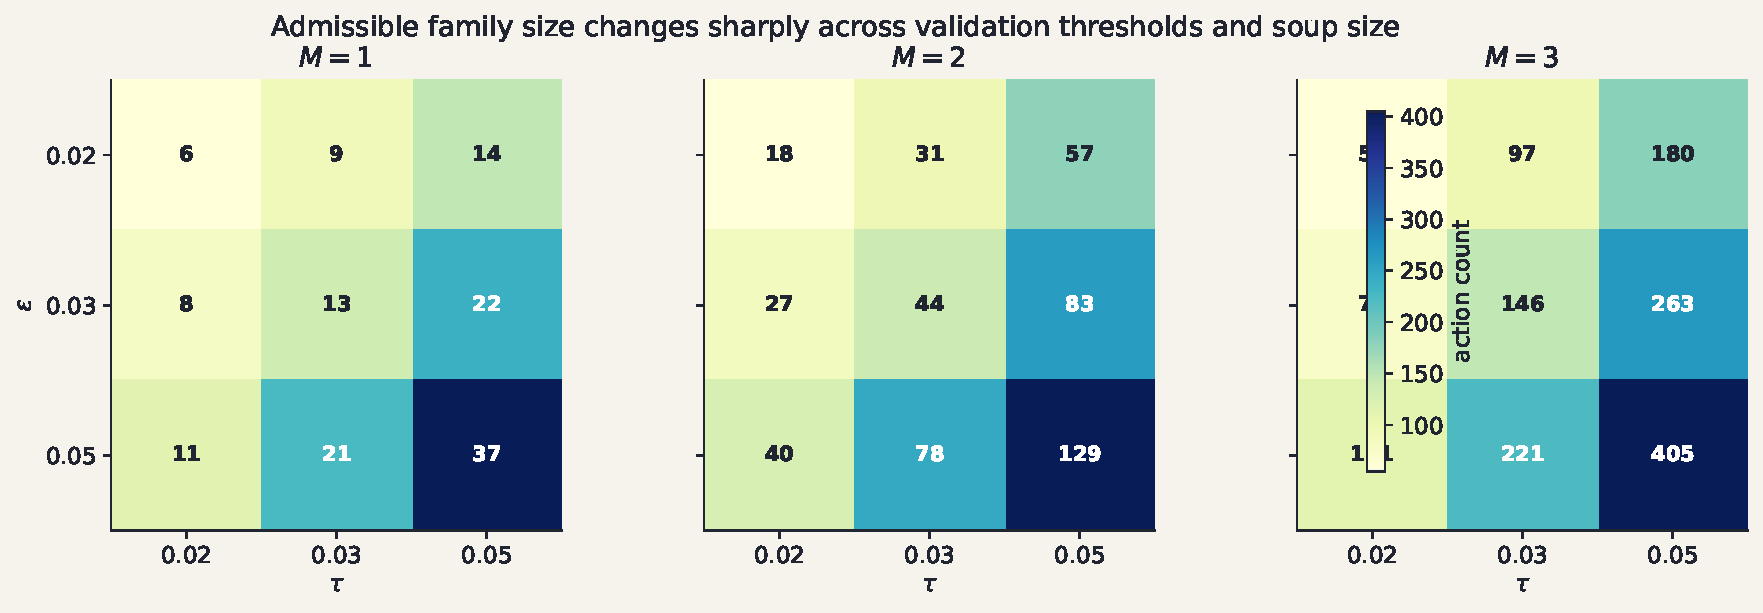
\includegraphics[width=0.88\linewidth]{figures/search_budget_frontier.pdf}
    \caption{\textbf{Why the search budget is part of the method.} The admissible-family restriction prevents the selector from drifting into intractable exact-search regimes while preserving a theorem-governed finite action union.}
    \label{fig:budget}
\end{figure}

\section{Theory}
\label{sec:theory}

\subsection{Population hidden-subpopulation regret}

Let \(P\) be the pooled source-support distribution over \(Z=(X,Y)\). For action \(S\), let \(\loss(Z;S)\in[0,1]\) denote the normalized population loss. Define the source-supported hidden-subpopulation family
\begin{equation}
    \cR_\alpha
    \triangleq
    \braces{
        r : \mathcal Z \to [0,\alpha^{-1}] :
        \EE_P[r(Z)] = 1
    }.
    \label{eq:population_reweightings}
\end{equation}
Each \(r\in\cR_\alpha\) induces \(P_r\) by \(dP_r = r\,dP\).

For admissible \(\gamma\in\Gamma_{\mathrm{adm}}(\cV)\), define the population regret of \(S\in\cA_\gamma(\cV)\) under \(r\in\cR_\alpha\) by
\begin{equation}
    \operatorname{Reg}^{(\gamma,\cV)}_r(S)
    \triangleq
    \EE_{P_r}[\loss(Z;S)]
    -
    \min_{S'\in\cA_\gamma(\cV)}
    \EE_{P_r}[\loss(Z;S')].
    \label{eq:population_regret}
\end{equation}
The family-indexed population objective is
\begin{equation}
    \Psi^{(\gamma,\cV)}_\alpha(S)
    \triangleq
    \sup_{r\in\cR_\alpha}
    \operatorname{Reg}^{(\gamma,\cV)}_r(S).
    \label{eq:population_objective}
\end{equation}

\begin{theorem}[Target-regret certificate]
\label{thm:certificate}
For every admissible \(\gamma\in\Gamma_{\mathrm{adm}}(\cV)\), every \(S\in\cA_\gamma(\cV)\), and every \(r\in\cR_\alpha\),
\begin{equation}
    \operatorname{Reg}^{(\gamma,\cV)}_r(S)
    \le
    \Psi^{(\gamma,\cV)}_\alpha(S).
    \label{eq:certificate}
\end{equation}
Consequently, the population minimizer in any admissible family minimizes the worst-case regret certificate over all source-supported hidden-subpopulation shifts of mass at least \(\alpha\).
\end{theorem}

\begin{proposition}[Population top-\(\alpha\) / \(\CVaR\) representation]
\label{prop:population_top_alpha}
Fix admissible \(\gamma\in\Gamma_{\mathrm{adm}}(\cV)\) and ordered pair \((S,S')\in\Omega_\gamma(\cV)\). Define
\begin{equation}
    R^{(\gamma,\cV)}_\alpha(S,S')
    \triangleq
    \sup_{r\in\cR_\alpha}
    \EE_{P_r}\!\left[\loss(Z;S)-\loss(Z;S')\right].
    \label{eq:population_pairwise}
\end{equation}
Then
\begin{equation}
    R^{(\gamma,\cV)}_\alpha(S,S')
    =
    \inf_{\eta\in\RR}
    \bracks{
        \eta + \frac{1}{\alpha}\EE\paren{\loss(Z;S)-\loss(Z;S')-\eta}_+
    }.
    \label{eq:population_cvar}
\end{equation}
Moreover,
\begin{equation}
    \Psi^{(\gamma,\cV)}_\alpha(S)
    =
    \max_{S'\in\cA_\gamma(\cV)}
    R^{(\gamma,\cV)}_\alpha(S,S').
    \label{eq:population_max_pair}
\end{equation}
\end{proposition}

\subsection{Finite-sample deviation over the admissible family union}

For admissible \(\gamma\in\Gamma_{\mathrm{adm}}(\cV)\), define the pairwise witness class
\begin{equation}
    \Omega_\gamma(\cV)
    \triangleq
    \braces{
        (S,S') :
        S,S'\in\cA_\gamma(\cV)
    },
    \qquad
    |\Omega_\gamma(\cV)| = |\cA_\gamma(\cV)|^2.
    \label{eq:pair_class}
\end{equation}

\begin{theorem}[Conditional finite-sample deviation]
\label{thm:deviation}
Condition on the validation split \(\cV\). With probability at least \(1-\delta\) over the support sample \(\cU\sim P^n\), the following holds simultaneously for every admissible \(\gamma\in\Gamma_{\mathrm{adm}}(\cV)\) and every \(S\in\cA_\gamma(\cV)\):
\begin{equation}
    \left|
        \widehat{\Psi}^{(\gamma,\cV)}_\alpha(S;\cU)
        -
        \Psi^{(\gamma,\cV)}_\alpha(S)
    \right|
    \le
    \operatorname{pen}_{\alpha,n,\delta}(\gamma;\cV),
    \label{eq:uniform_deviation}
\end{equation}
where \(\operatorname{pen}_{\alpha,n,\delta}\) is defined in Eq.~\eqref{eq:penalty}.
\end{theorem}

The dependence on \(|\cA_\gamma(\cV)|^2\) is not accidental. The regret of one action is measured relative to the best witness action in the same family, so the relevant finite object is an ordered pair class.

\begin{theorem}[Oracle inequality for the family-aware selector]
\label{thm:oracle}
Under the same event as Theorem~\ref{thm:deviation},
\begin{equation}
    \Psi^{(\widehat{\gamma}_\alpha,\cV)}_\alpha(\widehat{S}_\alpha)
    \le
    \inf_{\gamma\in\Gamma_{\mathrm{adm}}(\cV),\;S\in\cA_\gamma(\cV)}
    \bracks{
        \Psi^{(\gamma,\cV)}_\alpha(S)
        +
        2\,\operatorname{pen}_{\alpha,n,\delta}(\gamma;\cV)
    }.
    \label{eq:oracle}
\end{equation}
\end{theorem}

\begin{corollary}[Consistency conditional on the validation-defined admissible family]
\label{cor:consistency}
Fix \(\alpha,\delta,\Gamma_0,K_{\max}\), and condition on \(\cV\). If \(\Gamma_{\mathrm{adm}}(\cV)\) is nonempty, then
\begin{equation}
    \sup_{\gamma\in\Gamma_{\mathrm{adm}}(\cV),\,S\in\cA_\gamma(\cV)}
    \left|
        \widehat{\Psi}^{(\gamma,\cV)}_\alpha(S;\cU)
        -
        \Psi^{(\gamma,\cV)}_\alpha(S)
    \right|
    \xrightarrow[]{a.s.} 0
    \qquad \text{as } n\to\infty.
    \label{eq:consistency}
\end{equation}
If the unpenalized population objective over the admissible union has a unique minimizer
\[
    (\gamma^\star_\alpha,S^\star_\alpha)
    \in
    \argmin_{\gamma\in\Gamma_{\mathrm{adm}}(\cV),\,S\in\cA_\gamma(\cV)}
    \Psi^{(\gamma,\cV)}_\alpha(S)
\]
and a positive gap to every other admissible pair, then the selected pair \((\widehat{\gamma}_\alpha,\widehat{S}_\alpha)\) eventually identifies \((\gamma^\star_\alpha,S^\star_\alpha)\) almost surely.
\end{corollary}

\subsection{Comparison to interval-restricted selectors}

Many post-hoc DG selectors deploy soups from a contiguous interval family. In our notation, an interval-restricted family in admissible family \(\gamma\) is any subfamily
\begin{equation}
    \cI_\gamma(\cV)
    \subseteq
    \cA_\gamma(\cV)
    \label{eq:interval_subfamily}
\end{equation}
whose actions are contiguous in trajectory order.

\begin{corollary}[Interval-family domination on the \prism{} certificate]
\label{cor:interval}
For any admissible family \(\gamma\in\Gamma_{\mathrm{adm}}(\cV)\),
\begin{equation}
    \inf_{S\in\cA_\gamma(\cV)}
    \Psi^{(\gamma,\cV)}_\alpha(S)
    \le
    \inf_{I\in\cI_\gamma(\cV)}
    \Psi^{(\gamma,\cV)}_\alpha(I).
    \label{eq:interval_domination}
\end{equation}
Under the event of Theorem~\ref{thm:deviation},
\begin{equation}
    \Psi^{(\widehat{\gamma}_\alpha,\cV)}_\alpha(\widehat{S}_\alpha)
    \le
    \inf_{\gamma\in\Gamma_{\mathrm{adm}}(\cV),\,I\in\cI_\gamma(\cV)}
    \bracks{
        \Psi^{(\gamma,\cV)}_\alpha(I)
        +
        2\,\operatorname{pen}_{\alpha,n,\delta}(\gamma;\cV)
    }.
    \label{eq:interval_oracle}
\end{equation}
\end{corollary}

Corollary~\ref{cor:interval} is the clean theorem-level comparison to interval-based post-hoc selectors. It does \emph{not} prove unconditional empirical domination. It proves something narrower and defensible: when interval actions live inside the admissible \prism{} family, the \prism{} selector is no worse than the best such interval action on the \prism{} certificate, up to the same family complexity term.

\begin{figure}[t]
    \centering
    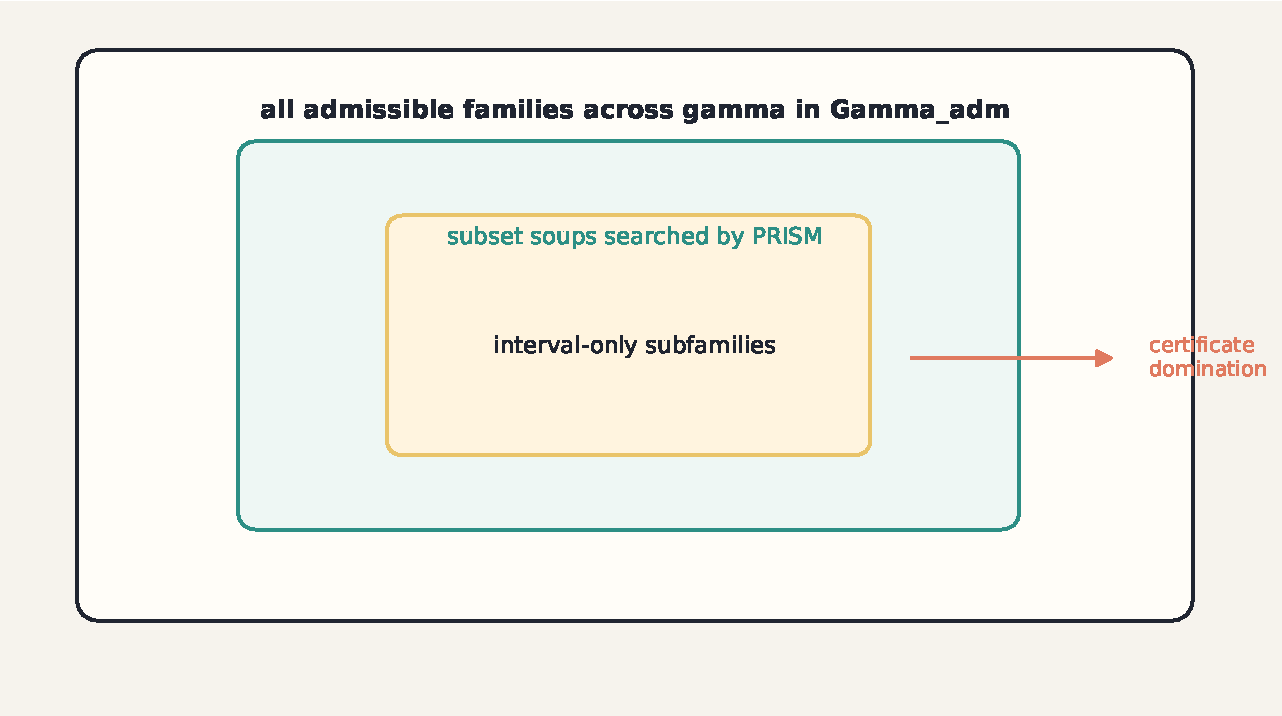
\includegraphics[width=0.88\linewidth]{figures/interval_domination.pdf}
    \caption{\textbf{Why interval selectors are a strict special case here.} Any contiguous interval family is a subfamily of the admissible subset soups searched by \prism{}. The theorem-level comparison is therefore a subfamily domination statement on the same certificate.}
    \label{fig:interval}
\end{figure}

\subsection{Monotonic robustness certificates}

\begin{proposition}[Monotonicity in \(\alpha\)]
\label{prop:alpha}
For every admissible family \(\gamma\in\Gamma_{\mathrm{adm}}(\cV)\) and every \(S\in\cA_\gamma(\cV)\), the map \(\alpha\mapsto \Psi^{(\gamma,\cV)}_\alpha(S)\) is nonincreasing on \((0,1]\).
\end{proposition}

This yields a robustness threshold at regret tolerance \(\tau_{\mathrm{reg}}>0\):
\begin{equation}
    \alpha^\star_{\tau_{\mathrm{reg}}}(\gamma,S)
    \triangleq
    \inf \braces{
        \alpha\in(0,1] :
        \Psi^{(\gamma,\cV)}_\alpha(S)\le \tau_{\mathrm{reg}}
    }.
    \label{eq:alpha_star}
\end{equation}
Smaller values of \(\alpha^\star_{\tau_{\mathrm{reg}}}\) certify robustness to smaller hidden subpopulations.

\begin{figure}[t]
    \centering
    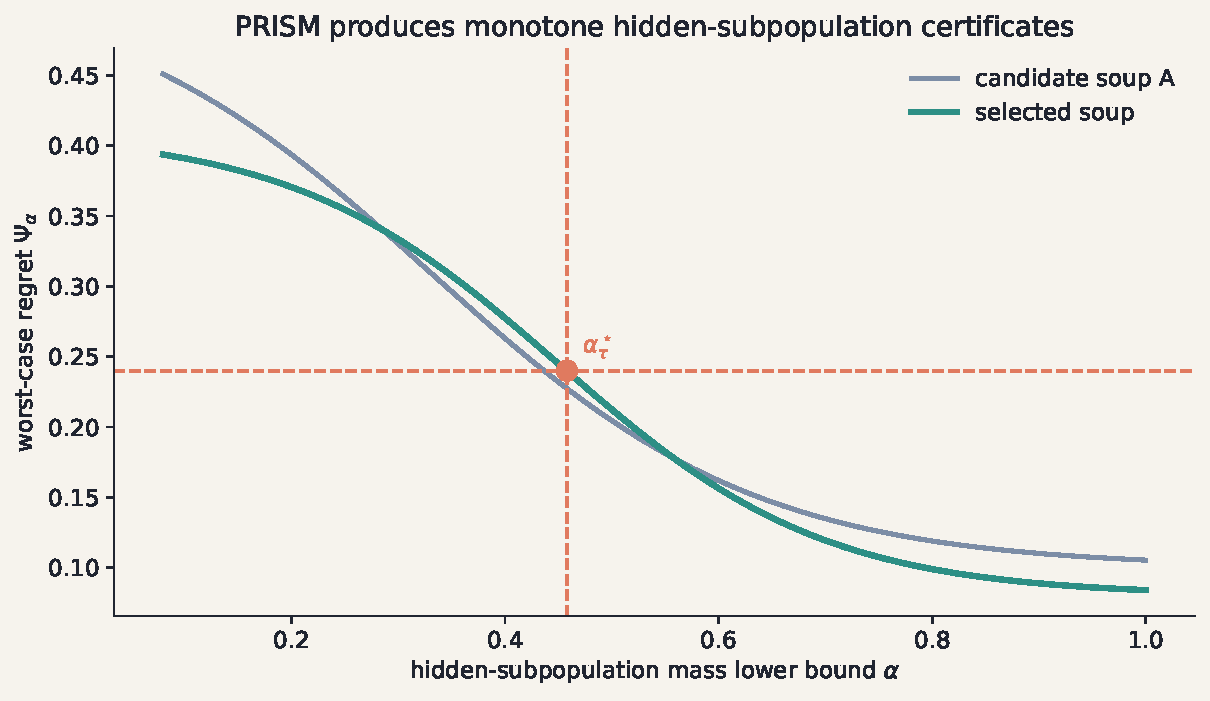
\includegraphics[width=0.82\linewidth]{figures/alpha_certificate_curve.pdf}
    \caption{\textbf{Monotone robustness certificate.} Because \(\Psi^{(\gamma,\cV)}_\alpha(S)\) decreases with \(\alpha\), every selected soup admits a threshold \(\alpha^\star\) at any chosen regret tolerance.}
    \label{fig:alpha_curve}
\end{figure}

\subsection{Why \prism{} can improve on raw within-family selection}

\begin{remark}[What the theory does and does not prove]
\label{rem:comparison}
The theory proves family-aware certificate control and domination over interval-restricted subfamilies on the \prism{} objective. It does \emph{not} prove unconditional empirical superiority to every flat-minima selector on every benchmark. That stronger claim would require assumptions about how closely the hidden-subpopulation certificate matches each benchmark’s true target shift.
\end{remark}

\section{Experimental Protocol and Published Context}
\label{sec:experiments}

This section records the empirical protocol and exact published benchmark context from prior work. The new \prism{} results are intentionally left as \TBD{} placeholders.

\subsection{Protocol}

The planned evaluation follows the standard DomainBed leave-one-domain-out protocol on PACS, VLCS, OfficeHome, TerraIncognita, and DomainNet \citep{gulrajani2021domainbed}. The base learner is a single dense source-pooled run. The held-out pooled source data are partitioned into validation and support subsets. The validation split defines admissible families, while the support split is reserved for hidden-subpopulation regret scoring.

The planned comparisons include:
\begin{itemize}[leftmargin=1.4em]
    \item plain \erm{};
    \item interval-based flat-minima selection;
    \item diverse or locality-aware averaging baselines;
    \item pretraining-aware DG methods with and without post-hoc selection;
    \item and ablations over \(\alpha\), \(K_{\max}\), \(\Gamma_0\), and the family prior.
\end{itemize}

\subsection{Published benchmark context}

Table~\ref{tab:published_context} records exact published numbers that define the current post-hoc DG context. These values are copied from the original papers and kept in their original reporting styles.

\begin{table}[t]
    \centering
    \small
    \caption{\textbf{Published DomainBed context from prior work.} The first block reproduces the reporting style of \citet{cha2021swad}; the second block reproduces the reporting style of \citet{cha2022miro}; the third block reproduces the reporting style of \citet{rame2022diwa}.}
    \label{tab:published_context}
    \setlength{\tabcolsep}{5pt}
    \begin{tabular}{lcccccc}
        \toprule
        Method & PACS & VLCS & OfficeHome & TerraInc & DomainNet & Avg. \\
        \midrule
        \erm{} \citep{cha2021swad} & 85.5 & 77.5 & 66.5 & 46.1 & 40.9 & 63.3 \\
        \swad{} \citep{cha2021swad} & 88.1 & 79.1 & 70.6 & 50.0 & 46.5 & 66.9 \\
        CORAL + \swad{} \citep{cha2021swad} & 88.3 & 78.9 & 71.3 & 51.0 & 46.8 & 67.3 \\
        \midrule
        \miro{} \citep{cha2022miro} & \(85.4\pm0.4\) & \(79.0\pm0.0\) & \(70.5\pm0.4\) & \(50.4\pm1.1\) & \(44.3\pm0.2\) & 65.9 \\
        \miro{} + \swad{} \citep{cha2022miro} & \(88.4\pm0.1\) & \(79.6\pm0.2\) & \(72.4\pm0.1\) & \(52.9\pm0.2\) & \(47.0\pm0.0\) & 68.1 \\
        \midrule
        \diwa{} (LP init, restricted \(M\le 20\)) \citep{rame2022diwa} & \(88.0\pm0.3\) & \(78.5\pm0.1\) & \(71.5\pm0.2\) & \(51.6\pm0.9\) & \(47.7\pm0.1\) & 67.5 \\
        \diwa{} (LP init, uniform \(M=20\)) \citep{rame2022diwa} & \(88.7\pm0.2\) & \(78.4\pm0.2\) & \(72.1\pm0.2\) & \(51.4\pm0.6\) & \(47.4\pm0.2\) & 67.6 \\
        \diwa{}$^\dagger$ (LP init, uniform \(M=60\)) \citep{rame2022diwa} & 89.0 & 78.6 & 72.8 & 51.9 & 47.7 & 68.0 \\
        \bottomrule
    \end{tabular}
\end{table}

\subsection{\prism{} reporting tables}

\begin{table}[t]
    \centering
    \small
    \caption{\textbf{Primary \prism{} reporting table.}}
    \label{tab:prism_tbd}
    \setlength{\tabcolsep}{7pt}
    \begin{tabular}{lcccccc}
        \toprule
        Method & PACS & VLCS & OfficeHome & TerraInc & DomainNet & Avg. \\
        \midrule
        \prism{} & \TBD & \TBD & \TBD & \TBD & \TBD & \TBD \\
        \prism{} + stronger backbone & \TBD & \TBD & \TBD & \TBD & \TBD & \TBD \\
        \prism{} + pretrained base & \TBD & \TBD & \TBD & \TBD & \TBD & \TBD \\
        \bottomrule
    \end{tabular}
\end{table}

\begin{table}[t]
    \centering
    \small
    \caption{\textbf{\prism{} ablation table.}}
    \label{tab:ablation_tbd}
    \setlength{\tabcolsep}{8pt}
    \begin{tabular}{lccc}
        \toprule
        Variant & PACS & Avg. & Comment \\
        \midrule
        \prism{} baseline & \TBD & \TBD & SRM over admissible families \\
        fixed family, no SRM & \TBD & \TBD & manual family choice \\
        smaller \(\alpha\) & \TBD & \TBD & sharper hidden-subpopulation adversary \\
        tighter \(K_{\max}\) & \TBD & \TBD & stronger tractability restriction \\
        interval-only subfamily & \TBD & \TBD & contiguous-action comparator \\
        \bottomrule
    \end{tabular}
\end{table}

\begin{table}[t]
    \centering
    \small
    \caption{\textbf{Certificate and compute reporting table.}}
    \label{tab:certificate_tbd}
    \setlength{\tabcolsep}{8pt}
    \begin{tabular}{lcccc}
        \toprule
        Variant & \(\alpha^\star_{\tau_{\mathrm{reg}}}\) & admissible families & scored actions & time \\
        \midrule
        \prism{} & \TBD & \TBD & \TBD & \TBD \\
        fixed family & \TBD & \TBD & \TBD & \TBD \\
        interval-only subfamily & \TBD & \TBD & \TBD & \TBD \\
        \bottomrule
    \end{tabular}
\end{table}

\section{Discussion}

\prism{} is intentionally narrow. It does not attempt to solve arbitrary DG shift. The population theorem is conditional on source-supported hidden-subpopulation reweightings. The validation barrier remains a locality modeling choice. And the finite-family theorems justify a family-aware selector, not universal domination over every competing heuristic.

Those restrictions are deliberate. The main point of \prism{} is alignment. The deployable object is a real soup. The witness class is the exact family from which that soup is drawn. The outer choice among admissible soup families is included in the selector rather than fixed by manual tuning. The resulting oracle inequality therefore speaks about the object the method actually deploys.

Several extensions remain open. Larger action families will require branch-and-bound or column-generation style search without changing the objective. Attribute-aware hidden-subpopulation families could replace the fully implicit reweighting class when auxiliary metadata are available. And a held-out-prior PAC-Bayes refinement remains attractive, but only once a regret-level stochastic theorem is written for the same object.

\section*{Acknowledgments}

This section is intentionally omitted for anonymous review.

\bibliographystyle{plainnat}
\bibliography{references}

\appendix

\section{Additional Visual Intuition}

\begin{figure}[h]
    \centering
    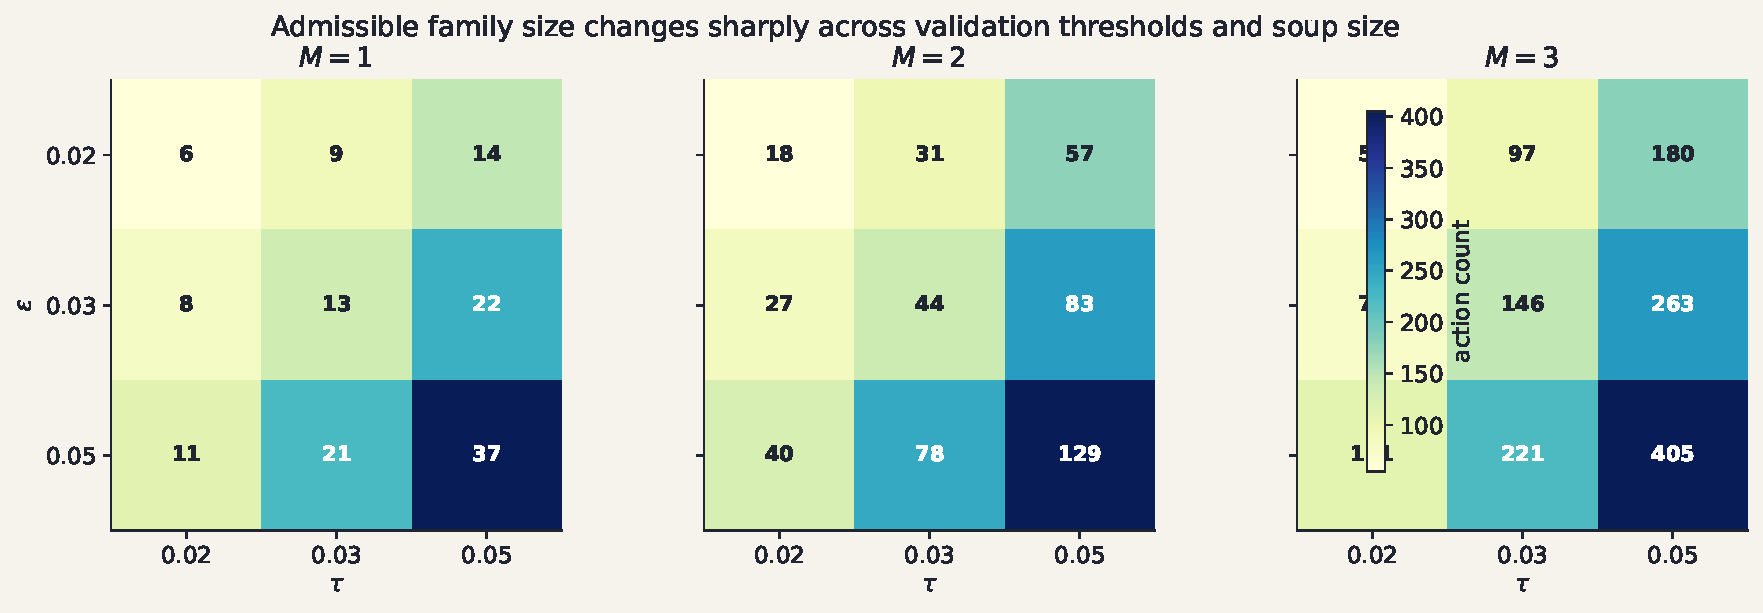
\includegraphics[width=0.88\linewidth]{figures/family_grid_heatmap.pdf}
    \caption{\textbf{Admissible family grid.} Different settings of validation width, locality, and soup size induce families of very different sizes. \prism{} reasons over these families explicitly instead of pretending one hand-picked family is the only relevant object.}
    \label{fig:grid}
\end{figure}

\section{Proofs}

\subsection{Proof of Proposition~\ref{prop:top_alpha}}

\begin{proof}
Fix admissible \(\gamma\in\Gamma_{\mathrm{adm}}(\cV)\) and \(S\in\cA_\gamma(\cV)\). Starting from Eq.~\eqref{eq:family_regret},
\begin{align}
    \widehat{\Psi}^{(\gamma,\cV)}_\alpha(S;\cU)
    &=
    \sup_{q\in\cQ_\alpha^n}
    \left[
        \sum_{i=1}^{n} q_i \loss_i(S)
        -
        \min_{S'\in\cA_\gamma(\cV)}
        \sum_{i=1}^{n} q_i \loss_i(S')
    \right]
    \nonumber\\
    &=
    \sup_{q\in\cQ_\alpha^n}
    \max_{S'\in\cA_\gamma(\cV)}
    \sum_{i=1}^{n} q_i\paren{\loss_i(S)-\loss_i(S')}
    \nonumber\\
    &=
    \max_{S'\in\cA_\gamma(\cV)}
    \sup_{q\in\cQ_\alpha^n}
    \sum_{i=1}^{n} q_i\paren{\loss_i(S)-\loss_i(S')},
    \label{eq:proof_swap}
\end{align}
because the outer maximization over \(S'\) is finite. This proves Eq.~\eqref{eq:family_top_alpha}.

Now fix \(v\in\RR^n\). By definition, \(\Top_\alpha(v)\) is a linear optimization over the compact polytope \(\cQ_\alpha^n\), so the supremum is attained at an extreme point. Standard linear-program duality for the constraints \(q\ge 0\), \(\sum_i q_i=1\), and \(q_i\le 1/(\alpha n)\) yields
\[
    \Top_\alpha(v)
    =
    \inf_{\eta\in\RR}
    \left[
        \eta + \frac{1}{\alpha n}\sum_{i=1}^{n}(v_i-\eta)_+
    \right].
\]
Substituting \(v=\loss(S)-\loss(S')\) gives the exact empirical-\(\CVaR\) form of the regret objective.
\end{proof}

\subsection{Proof of Proposition~\ref{prop:termination}}

\begin{proof}
The grid \(\Gamma_0\) is finite by construction, so \(\Gamma_{\mathrm{adm}}(\cV)\subseteq\Gamma_0\) is finite as well. For each admissible \(\gamma\), the action family \(\cA_\gamma(\cV)\) is finite. Algorithm~\ref{alg:prism} enumerates every admissible family and every action inside each family, evaluates the exact score in Eq.~\eqref{eq:prism_selector}, and returns a minimizer. Therefore it terminates after finitely many operations and returns a global minimizer.

Equation~\eqref{eq:total_actions} is immediate from summing the family sizes over admissible \(\gamma\). For each admissible family, computing family-indexed regrets from pairwise top-\(\alpha\) gaps requires \(O(n|\cA_\gamma(\cV)|^2)\) operations. Summing over admissible families gives Eq.~\eqref{eq:complexity}.
\end{proof}

\subsection{Proof of Theorem~\ref{thm:certificate}}

\begin{proof}
Fix admissible \(\gamma\), action \(S\in\cA_\gamma(\cV)\), and reweighting \(r\in\cR_\alpha\). By definition,
\[
    \operatorname{Reg}^{(\gamma,\cV)}_r(S)
    =
    \EE_{P_r}[\loss(Z;S)]
    -
    \min_{S'\in\cA_\gamma(\cV)}
    \EE_{P_r}[\loss(Z;S')].
\]
But \(\Psi^{(\gamma,\cV)}_\alpha(S)\) is the supremum of this quantity over all \(r'\in\cR_\alpha\). Therefore
\[
    \operatorname{Reg}^{(\gamma,\cV)}_r(S)
    \le
    \sup_{r'\in\cR_\alpha}
    \operatorname{Reg}^{(\gamma,\cV)}_{r'}(S)
    =
    \Psi^{(\gamma,\cV)}_\alpha(S).
\]
\end{proof}

\subsection{Proof of Proposition~\ref{prop:population_top_alpha}}

\begin{proof}
Fix admissible \(\gamma\in\Gamma_{\mathrm{adm}}(\cV)\) and \((S,S')\in\Omega_\gamma(\cV)\). Let
\[
    \Delta(Z)
    \triangleq
    \loss(Z;S)-\loss(Z;S') \in [-1,1].
\]
By definition of \(\cR_\alpha\),
\[
    R^{(\gamma,\cV)}_\alpha(S,S')
    =
    \sup\braces{
        \EE_P[r(Z)\Delta(Z)] :
        0\le r\le \alpha^{-1},\;
        \EE_P[r]=1
    }.
\]
This is the population analogue of the capped-simplex maximization in the empirical problem. Consider the convex program
\[
    \sup_r \EE_P[r\Delta]
    \quad
    \text{s.t. }
    0\le r\le \alpha^{-1},
    \;
    \EE_P[r]=1.
\]
Introduce a Lagrange multiplier \(\eta\in\RR\) for the equality constraint \(\EE_P[r]=1\). The Lagrangian is
\[
    \mathcal L(r,\eta)
    =
    \EE_P[r\Delta] - \eta(\EE_P[r]-1)
    =
    \eta + \EE_P\!\left[r(\Delta-\eta)\right].
\]
For fixed \(\eta\), maximizing pointwise over \(r(z)\in[0,\alpha^{-1}]\) gives
\[
    \sup_{0\le r\le \alpha^{-1}} r(z)\,(\Delta(z)-\eta)
    =
    \frac{1}{\alpha}(\Delta(z)-\eta)_+.
\]
Hence the dual objective is
\[
    \eta + \frac{1}{\alpha}\EE_P(\Delta-\eta)_+.
\]
Strong duality holds because the primal is feasible and convex, so
\[
    R^{(\gamma,\cV)}_\alpha(S,S')
    =
    \inf_{\eta\in\RR}
    \bracks{
        \eta + \frac{1}{\alpha}\EE_P(\Delta-\eta)_+
    },
\]
which proves Eq.~\eqref{eq:population_cvar}.

Now expand the family-indexed population regret:
\begin{align*}
    \Psi^{(\gamma,\cV)}_\alpha(S)
    &=
    \sup_{r\in\cR_\alpha}
    \left[
        \EE_{P_r}\loss(Z;S)
        -
        \min_{T\in\cA_\gamma(\cV)} \EE_{P_r}\loss(Z;T)
    \right]
    \\
    &=
    \sup_{r\in\cR_\alpha}
    \max_{T\in\cA_\gamma(\cV)}
    \EE_{P_r}\!\left[\loss(Z;S)-\loss(Z;T)\right].
\end{align*}
Because the witness family is finite, we may swap the outer supremum and the finite maximum:
\[
    \Psi^{(\gamma,\cV)}_\alpha(S)
    =
    \max_{T\in\cA_\gamma(\cV)}
    \sup_{r\in\cR_\alpha}
    \EE_{P_r}\!\left[\loss(Z;S)-\loss(Z;T)\right]
    =
    \max_{T\in\cA_\gamma(\cV)}
    R^{(\gamma,\cV)}_\alpha(S,T),
\]
which proves Eq.~\eqref{eq:population_max_pair}.
\end{proof}

\subsection{Proof of Theorem~\ref{thm:deviation}}

\begin{proof}
Condition on \(\cV\), and fix admissible \(\gamma\in\Gamma_{\mathrm{adm}}(\cV)\). For ordered pair \(\omega=(S,S')\in\Omega_\gamma(\cV)\), define the gap random variable
\[
    \Delta_\omega(Z)
    \triangleq
    \loss(Z;S)-\loss(Z;S') \in [-1,1].
\]
Using Proposition~\ref{prop:top_alpha} and Proposition~\ref{prop:population_top_alpha}, the empirical and population pairwise regret terms are
\begin{align}
    \widehat{R}_\alpha(\omega)
    &\triangleq
    \inf_{\eta\in\RR}
    \left[
        \eta + \frac{1}{\alpha n}\sum_{i=1}^{n}(\Delta_\omega(Z_i)-\eta)_+
    \right],
    \label{eq:emp_pair}
    \\
    R_\alpha(\omega)
    &\triangleq
    \inf_{\eta\in\RR}
    \left[
        \eta + \frac{1}{\alpha}\EE(\Delta_\omega(Z)-\eta)_+
    \right].
    \label{eq:pop_pair}
\end{align}

Because \(\Delta_\omega(Z)\in[-1,1]\), the infimum may be restricted to \(\eta\in[-1,1]\): outside this interval, replacing \(\eta\) by the nearest endpoint cannot increase the objective. Let
\[
    \Phi_{\omega,\eta}(Z)
    \triangleq
    \eta + \frac{1}{\alpha}(\Delta_\omega(Z)-\eta)_+.
\]
For \(\eta\in[-1,1]\), we have
\[
    -1 \le \Phi_{\omega,\eta}(Z) \le 1 + \frac{2}{\alpha},
\]
so its range length is at most \(2(1+\alpha^{-1})\). By Hoeffding's inequality, for any fixed \((\omega,\eta)\) and any \(u>0\),
\[
    \PP\!\left(
        \left|
            \frac{1}{n}\sum_{i=1}^{n}\Phi_{\omega,\eta}(Z_i)
            -
            \EE\Phi_{\omega,\eta}(Z)
        \right|
        >
        \left(1+\frac{1}{\alpha}\right)\sqrt{\frac{2u}{n}}
    \right)
    \le
    2e^{-u}.
\]

Now cover \([-1,1]\) by the grid
\[
    \Xi_n \triangleq \braces{-1,-1+\tfrac1n,\ldots,1}
\]
of size at most \(2n+1\). Since \(x\mapsto (x-\eta)_+\) is \(1\)-Lipschitz in \(\eta\), the map \(\eta\mapsto \Phi_{\omega,\eta}(Z)\) is \((1+\alpha^{-1})\)-Lipschitz uniformly in \(Z\). Therefore, for any \(\eta\in[-1,1]\), there exists \(\eta_0\in\Xi_n\) with \(|\eta-\eta_0|\le 1/n\) and
\[
    \left|
        \Phi_{\omega,\eta}(Z)-\Phi_{\omega,\eta_0}(Z)
    \right|
    \le
    \left(1+\frac{1}{\alpha}\right)\frac{1}{n}.
\]
Hence
\begin{align}
    \sup_{\eta\in[-1,1]}
    \left|
        \frac{1}{n}\sum_{i=1}^{n}\Phi_{\omega,\eta}(Z_i)
        -
        \EE\Phi_{\omega,\eta}(Z)
    \right|
    &\le
    \max_{\eta_0\in\Xi_n}
    \left|
        \frac{1}{n}\sum_{i=1}^{n}\Phi_{\omega,\eta_0}(Z_i)
        -
        \EE\Phi_{\omega,\eta_0}(Z)
    \right|
    \nonumber\\
    &\qquad +
    2\left(1+\frac{1}{\alpha}\right)\frac{1}{n}.
    \label{eq:net_bound}
\end{align}

Apply the fixed-\((\omega,\eta_0)\) Hoeffding bound to all \((\omega,\eta_0)\in \Omega_\gamma(\cV)\times\Xi_n\), allocating failure probability \(\delta \pi_\Gamma(\gamma)\). Since \(|\Omega_\gamma(\cV)|=|\cA_\gamma(\cV)|^2\), a union bound yields that with probability at least \(1-\delta\pi_\Gamma(\gamma)\),
\begin{align}
    \sup_{\omega\in\Omega_\gamma(\cV)}
    \sup_{\eta\in[-1,1]}
    \left|
        \frac{1}{n}\sum_{i=1}^{n}\Phi_{\omega,\eta}(Z_i)
        -
        \EE\Phi_{\omega,\eta}(Z)
    \right|
    \le
    \operatorname{pen}_{\alpha,n,\delta}(\gamma;\cV).
    \label{eq:family_dev}
\end{align}
Because \(|\inf f - \inf g|\le \sup |f-g|\), Eq.~\eqref{eq:family_dev} implies
\[
    \sup_{\omega\in\Omega_\gamma(\cV)}
    \left|
        \widehat{R}_\alpha(\omega) - R_\alpha(\omega)
    \right|
    \le
    \operatorname{pen}_{\alpha,n,\delta}(\gamma;\cV).
\]
Finally, \(\widehat{\Psi}^{(\gamma,\cV)}_\alpha(S;\cU)=\max_{S'}\widehat{R}_\alpha(S,S')\) and \(\Psi^{(\gamma,\cV)}_\alpha(S)=\max_{S'}R_\alpha(S,S')\). A maximum over finitely many terms cannot increase the deviation bound. Applying another union bound across \(\gamma\) using the prior allocation \(\pi_\Gamma(\gamma)\) proves the simultaneous result.
\end{proof}

\subsection{Proof of Theorem~\ref{thm:oracle}}

\begin{proof}
Work on the event of Theorem~\ref{thm:deviation}. By definition of the selector,
\[
    \widehat{\Psi}^{(\widehat{\gamma}_\alpha,\cV)}_\alpha(\widehat{S}_\alpha;\cU)
    +
    \operatorname{pen}_{\alpha,n,\delta}(\widehat{\gamma}_\alpha;\cV)
    \le
    \widehat{\Psi}^{(\gamma,\cV)}_\alpha(S;\cU)
    +
    \operatorname{pen}_{\alpha,n,\delta}(\gamma;\cV)
\]
for every admissible \(\gamma\) and every \(S\in\cA_\gamma(\cV)\). Using Theorem~\ref{thm:deviation} on the left and right,
\begin{align*}
    \Psi^{(\widehat{\gamma}_\alpha,\cV)}_\alpha(\widehat{S}_\alpha)
    &\le
    \widehat{\Psi}^{(\widehat{\gamma}_\alpha,\cV)}_\alpha(\widehat{S}_\alpha;\cU)
    +
    \operatorname{pen}_{\alpha,n,\delta}(\widehat{\gamma}_\alpha;\cV)
    \\
    &\le
    \widehat{\Psi}^{(\gamma,\cV)}_\alpha(S;\cU)
    +
    \operatorname{pen}_{\alpha,n,\delta}(\gamma;\cV)
    \\
    &\le
    \Psi^{(\gamma,\cV)}_\alpha(S)
    +
    2\,\operatorname{pen}_{\alpha,n,\delta}(\gamma;\cV).
 \end{align*}
Taking the infimum over admissible \(\gamma,S\) yields Eq.~\eqref{eq:oracle}.
\end{proof}

\subsection{Proof of Corollary~\ref{cor:consistency}}

\begin{proof}
For fixed admissible \(\gamma\), the penalty \(\operatorname{pen}_{\alpha,n,\delta}(\gamma;\cV)\) vanishes as \(n\to\infty\). By the proof of Theorem~\ref{thm:deviation}, the uniform deviation over each finite family also converges almost surely to zero by the strong law on the finite grid, and the admissible family union is finite conditional on \(\cV\). This proves Eq.~\eqref{eq:consistency}.

Because the admissible family union is finite conditional on \(\cV\), the penalties \(\operatorname{pen}_{\alpha,n,\delta}(\gamma;\cV)\) vanish uniformly over admissible \(\gamma\). If the unpenalized population objective has a unique minimizer with positive gap, then for all sufficiently large \(n\), the sum of the uniform deviation and the maximum penalty is smaller than half that gap. At that point no other admissible pair can beat \((\gamma^\star_\alpha,S^\star_\alpha)\), so the selected pair eventually identifies it almost surely.
\end{proof}

\subsection{Proof of Corollary~\ref{cor:interval}}

\begin{proof}
For fixed admissible \(\gamma\), the interval family \(\cI_\gamma(\cV)\) is a subset of \(\cA_\gamma(\cV)\). Therefore
\[
    \inf_{S\in\cA_\gamma(\cV)}
    \Psi^{(\gamma,\cV)}_\alpha(S)
    \le
    \inf_{I\in\cI_\gamma(\cV)}
    \Psi^{(\gamma,\cV)}_\alpha(I),
 \]
which proves Eq.~\eqref{eq:interval_domination}. Equation~\eqref{eq:interval_oracle} then follows by restricting the infimum in Theorem~\ref{thm:oracle} to interval actions.
\end{proof}

\subsection{Proof of Proposition~\ref{prop:alpha}}

\begin{proof}
If \(0<\alpha_1\le \alpha_2\le 1\), then \(\cR_{\alpha_2}\subseteq \cR_{\alpha_1}\) because the pointwise cap \(r\le \alpha_2^{-1}\) is stricter. Therefore for every admissible \(\gamma\) and every \(S\in\cA_\gamma(\cV)\),
\[
    \Psi^{(\gamma,\cV)}_{\alpha_2}(S)
    =
    \sup_{r\in\cR_{\alpha_2}}
    \operatorname{Reg}^{(\gamma,\cV)}_r(S)
    \le
    \sup_{r\in\cR_{\alpha_1}}
    \operatorname{Reg}^{(\gamma,\cV)}_r(S)
    =
    \Psi^{(\gamma,\cV)}_{\alpha_1}(S).
\]
\end{proof}

\section{High-Level Explanation}

\paragraph{What problem is \prism{} solving?}
After training one model, we usually have many checkpoints saved along the way. The question is: which final model should we actually use? Some older methods pick a single checkpoint or average a hand-chosen interval of checkpoints. \prism{} says we should do something more principled: compare many possible checkpoint-soup families and pick the one that is safest against hidden hard groups of examples, while also being careful not to trust a huge flexible family unless it really earns that trust on held-out data.

\paragraph{What does “hidden-subpopulation regret” mean?}
Imagine there is some unknown subgroup inside the source data that is especially hard, like a small style, lighting condition, or shape pattern. We do not know its label. \prism{} pretends an adversary is allowed to focus on any subgroup that is at least a certain size. For each candidate soup, it asks: how much worse is this soup than the best soup from the same family on that subgroup? That performance gap is regret. Small regret means the soup is hard to embarrass by any sufficiently large hidden subgroup.

\paragraph{What makes the new version different?}
The big change is that \prism{} no longer assumes we already know the right family of soups to search. It compares many validation-defined families and adds an Occam penalty for larger ones. So it is not just saying “find the best soup in one chosen family.” It is saying “find the best soup while also accounting for how complicated the search family was.” That is the structural-risk-minimization part.

\paragraph{What do the theorems actually prove?}
They prove that the objective has an exact tail-risk form, that the exhaustive search returns the true minimizer over the searched families, that the empirical score stays close to the population score with high probability, and that the selected family-action pair is nearly as good as the best admissible pair up to the explicit penalty. They also prove a clean comparison to interval-only methods: if those methods search a strict subfamily of soups that \prism{} also considers, then \prism{} is never worse on its own certificate than the best interval action from that same subfamily.

\paragraph{What do the theorems not prove?}
They do not prove that \prism{} will always beat every existing method on every benchmark. That would require stronger assumptions about the real test shift. What they do prove is that \prism{} is aligned with a richer and more honest objective than interval-only post-hoc selection, and that it controls the statistical price of searching over multiple soup families instead of pretending that one hand-picked family was the only reasonable one.

\end{document}
